\begin{sepframe}{History}
  {\scriptsize{A little bit of contextual information}}

\end{sepframe}

\begin{frame}[fragile,c]
  \makebox[\linewidth]{\includegraphics[width=\paperwidth, height=\paperheight]{src/session/history/resources/diagram.pdf}}

  \note[item]{
    Let's dive in the next chapter, we are going to do a brief history
    of programming languages and where we are coming from before diving into
    complexity and the rest.
  }
  \note[item]{
    I do not promise you to reach the ultimate sophistication to your code,
    but merely to open some doors to some extent.
  }

  \note[item]{
    What you see here in this horrendous and cumbersome slide is a graph
    where nodes represent programming languages. The edges are basically
    representing a relation between them. The relation here is
    "influenced by", so basically this language has been influenced by
    another.
  }

  \note[item]{
    We can see that there are many links and relations.
  }

  \note[item]{
    Let's me make a point about programming languages types and paradigms.
  }
\end{frame}

\begin{frame}
  \frametitle{History}
  \framesubtitle{Programming languages paradigms}

  \begin{itemize}[<+->]
    \item \textbf{O}bject \textbf{O}riented \textbf{P}rogramming
    \item \textbf{F}unctional \textbf{P}rogramming
    \item \textbf{I}mperative \textbf{P}rogramming
  \end{itemize}

  \note[item]{
    There are many programming languages paradigms, we are only going to
    discuss about a few of them.
  }

  \note[item]{
    The OOP paradigm, where software is designed around data structure and
    classes of objects.
  }

  \note[item]{
    The functional programming is basically a paradigm where programs are
    constructed by composing and applying functions only.
    This is also a sub-paradigm of the declarative paradigm which focus on
    describing "what" the program must accomplish rather than describing
    "how" to accomplish it.
  }

  \note[item]{
    And last but not least, the imperative programming paradigm. "Imperative"
    comes from latin word "imperare" which means "to command". This paradigm is
    made up of clear and well defined sequence of instructions. So basically a
    program is a series of command which specify what the computer has to do and
    when in order to achieve a desired result. To control the commands,
    control structures such as conditions and loops are existing.
  }
\end{frame}

{
\usebackgroundtemplate{
  \vbox to \paperheight{\vfil\hbox to \paperwidth{\hfil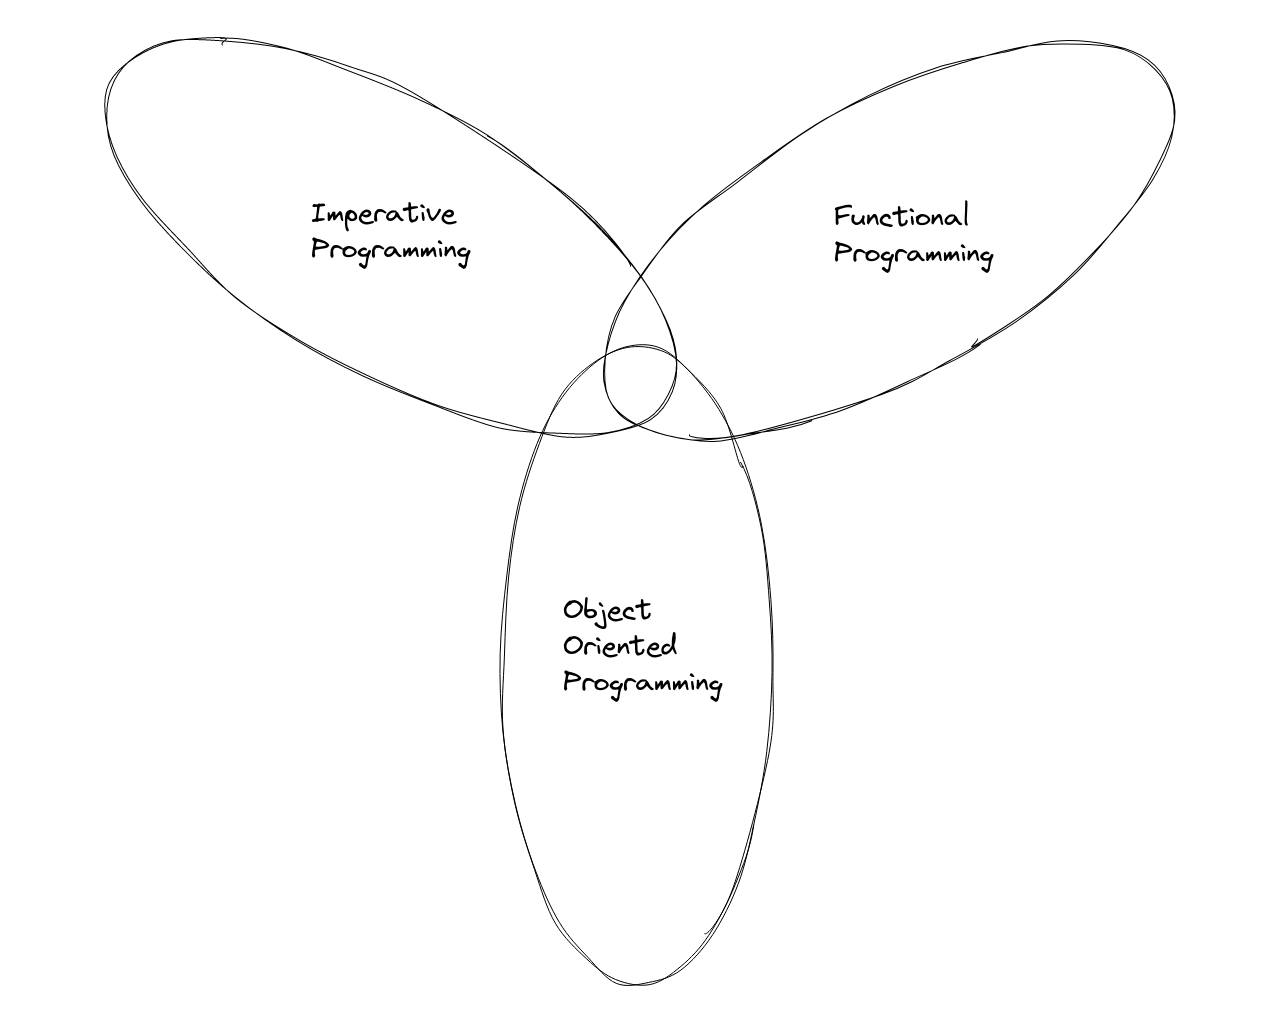
\includegraphics[keepaspectratio=true, width=\paperwidth, height=\paperheight]{src/session/history/resources/venn.png}\hfil}\vfil}
}
\begin{frame}

  \note[item]{
    Maybe all of this is ringing a bell? No?
    Keep in mind that these paradigms are not mutually exclusive, they can
    be used together without any issues.
  }

  \note[item]{
    If you do Typescript, PHP, Java... you are actually mixing all these
    paradigm most probably already. Some of use are more in one side than
    another.
  }

  \note[item]{
    From what I've seen so far until now along those years is that the trend
    is definitely to be more in the imperative way of programming.
  }

  \note[item]{
    My ultimate personal goal is to move the lines and trends by moving from
    imperative programming to functional programming for many reasons.
  }

\end{frame}
}

\begin{frame}[fragile,c]
  \frametitle{History}
  \framesubtitle{\textbf{I}mperative \textbf{P}rogramming}

  \makebox[\linewidth]{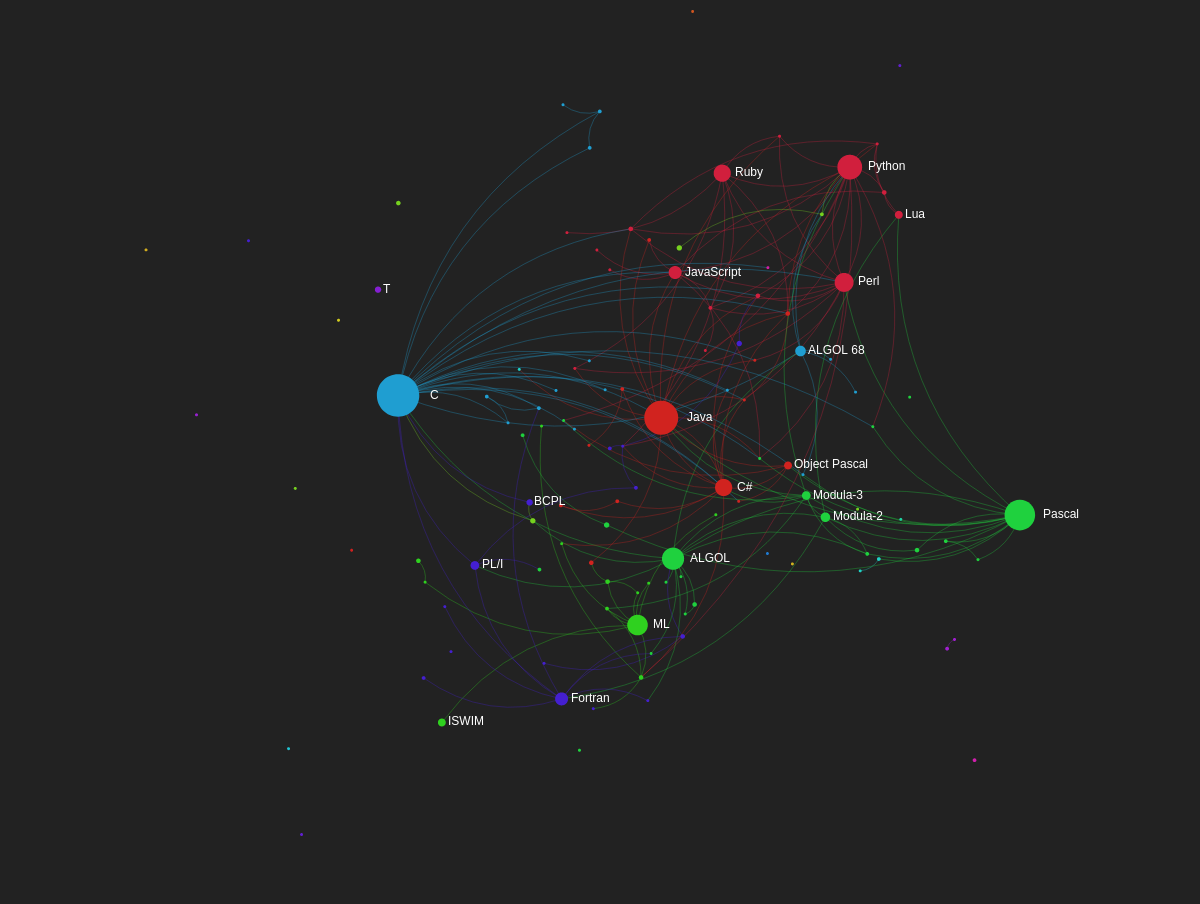
\includegraphics[width=\paperwidth, height=\paperheight]{src/session/history/resources/ip.png}}

  \note[item]{
    Look at this graph showing imperative programming languages.
  }

  \note[item]{
    We can see that a lot of languages inherit from C, Java, Pascal.
  }

  \note[item]{
    PHP is here (show where PHP is on the graph), and has been influenced by
    them.
    This is why the construction of some statements are similar. Actually
    a lot of things are similar when you think about it.
    It also means that PHP inherited from features of these languages.
  }
\end{frame}

\begin{frame}[fragile,c]
  \lstinputlisting{src/session/history/resources/oop.js}

  \note[item]{
    Have a look at this snippet.
  }

  \note[item]{
    Can you guess the paradigm?
  }

  \note[item]{
    I will not keep the suspense any longer, but in case you haven't seen it
    this Javascript snippet is computing odd numbers from a pre-defined list
    of numbers.
    Ok I know that there are many other ways to do that, but this example is
    actually a trivial example to show what imperative programming is.
    We don't basically tell the program to compute odd numbers, we actually
    "command" each line to do a particular thing, and in the end, it
    computes odd numbers.
  }
\end{frame}

\begin{frame}[fragile,c]
  \frametitle{History}
  \framesubtitle{\textbf{F}unctional \textbf{P}rogramming}

  \makebox[\linewidth]{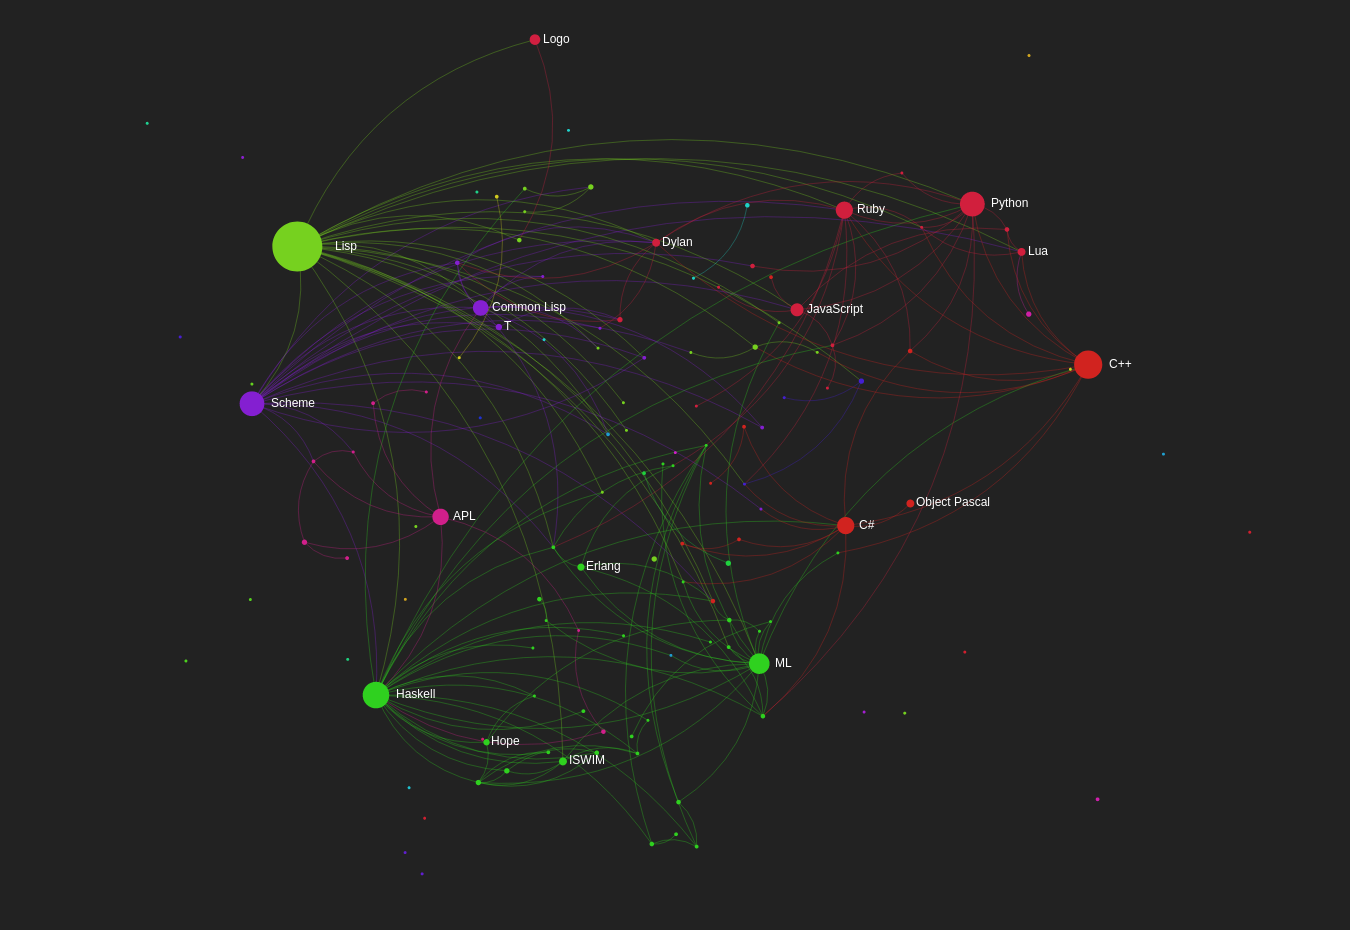
\includegraphics[width=\paperwidth, height=\paperheight]{src/session/history/resources/fp.png}}

  \note[item]{
    Let's now check the graph of functional programming paradigm...
  }

  \note[item]{
    No, PHP is not even displayed here.
  }
\end{frame}

\begin{frame}[fragile,c]
  \lstinputlisting{src/session/history/resources/fp.js}

  \note[item]{
    If we rewrite the previous Javascript snippet in functional programming
    paradigm, we have this.
  }

  \note[item]{
    Yes, it's shorter. When a piece of code is shorter, it's usually less
    prone to bugs and less maintenance ! I said usually.
    In this snippet, each lines has a different meaning, and everything is
    properly scoped, nothing is mixed up.
    First line is the input.
    Second line is a function which takes one array parameter and return an
    array.
    Third line is printing the result of the input applied to the function.
    Pretty simple, no?
  }
\end{frame}

\begin{frame}[fragile,c]
  \frametitle{History}
  \framesubtitle{\textbf{O}bject \textbf{O}riented \textbf{P}rogramming}

  \makebox[\linewidth]{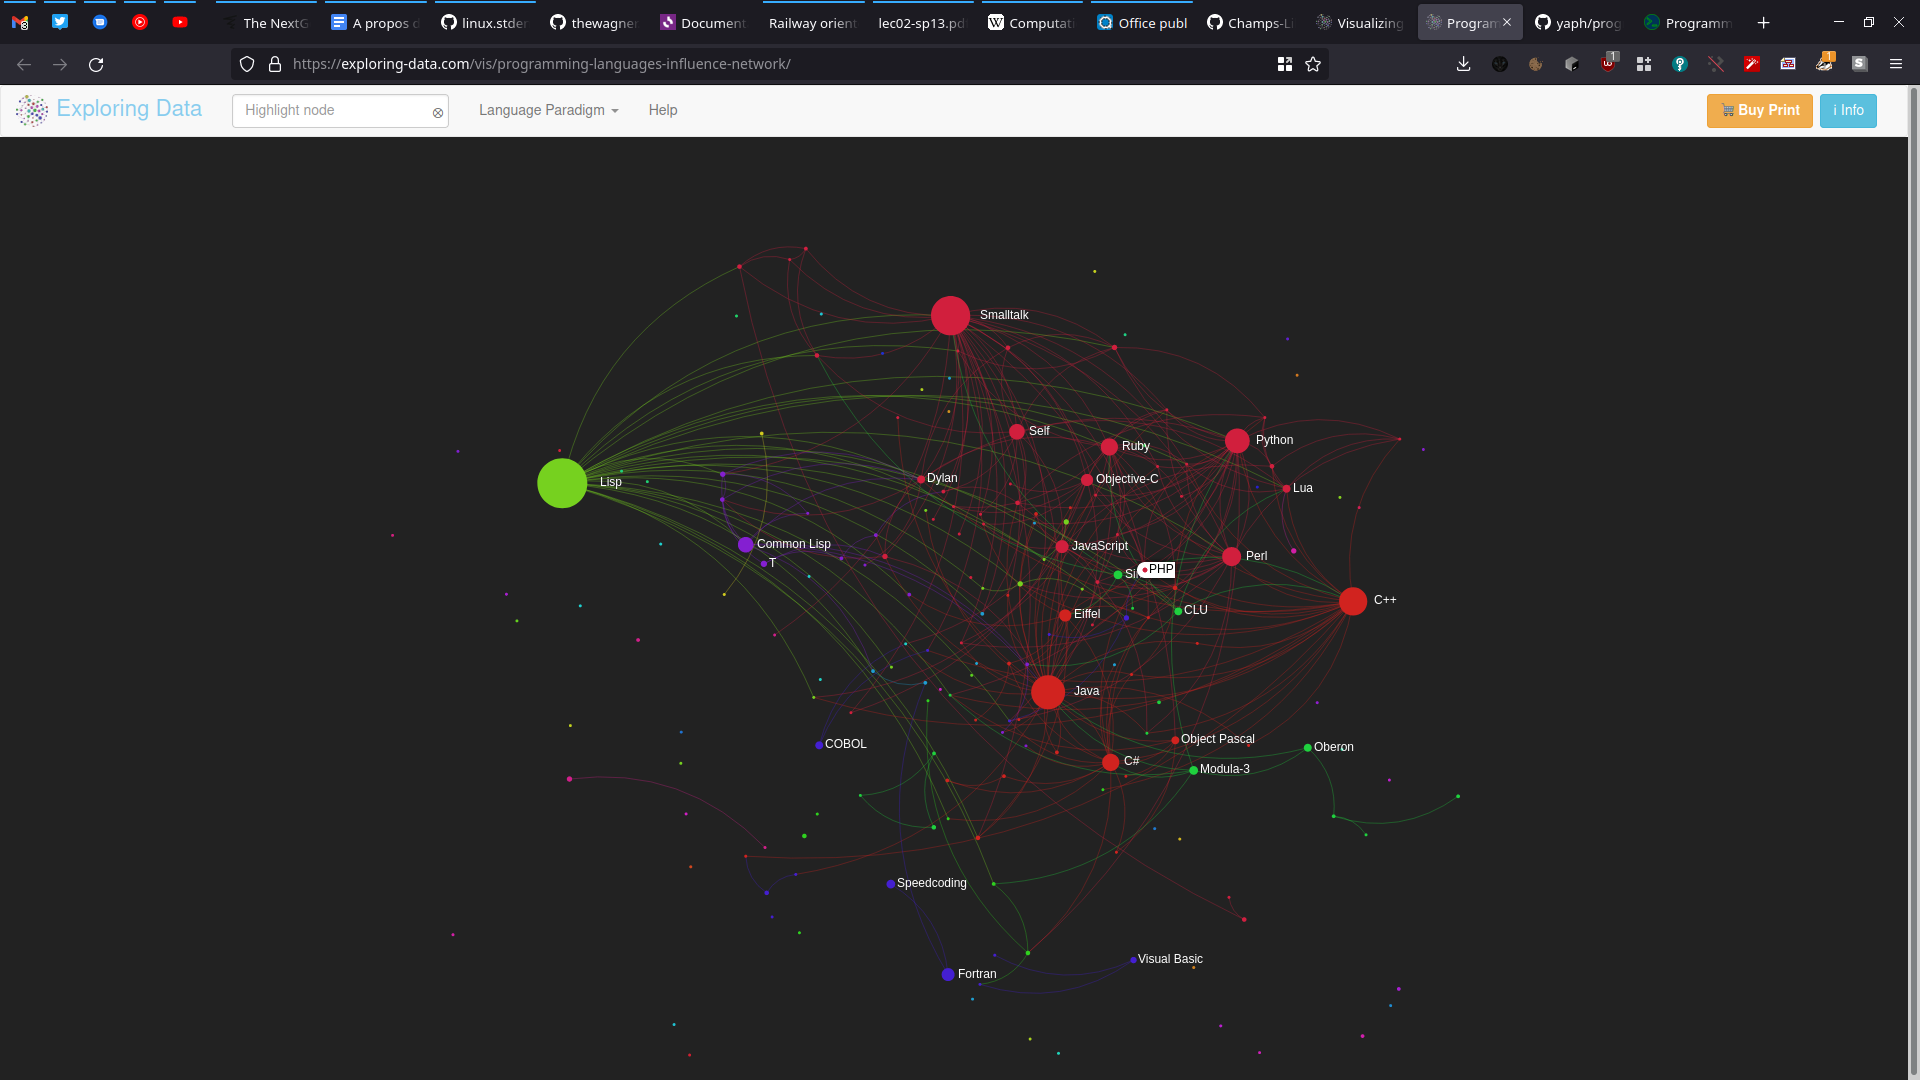
\includegraphics[width=\paperwidth, height=\paperheight]{src/session/history/resources/oop.png}}

  \note[item]{
    This last graph shows the OOP paradigm and its influence.
  }

  \note[item]{
    We can see PHP there.
  }

  \note[item]{
    We also see that Lisp has influenced a lot of languages out there, but not
    directly PHP.
  }
\end{frame}

\begin{frame}
  \centering
  \Huge What about PHP?

  \note[item]{
    And what about PHP in this landscape?
    As we can see here, PHP has been influenced by multi-paradigms
    languages.
  }
\end{frame}

\begin{frame}[plain]
  \makebox[\linewidth]{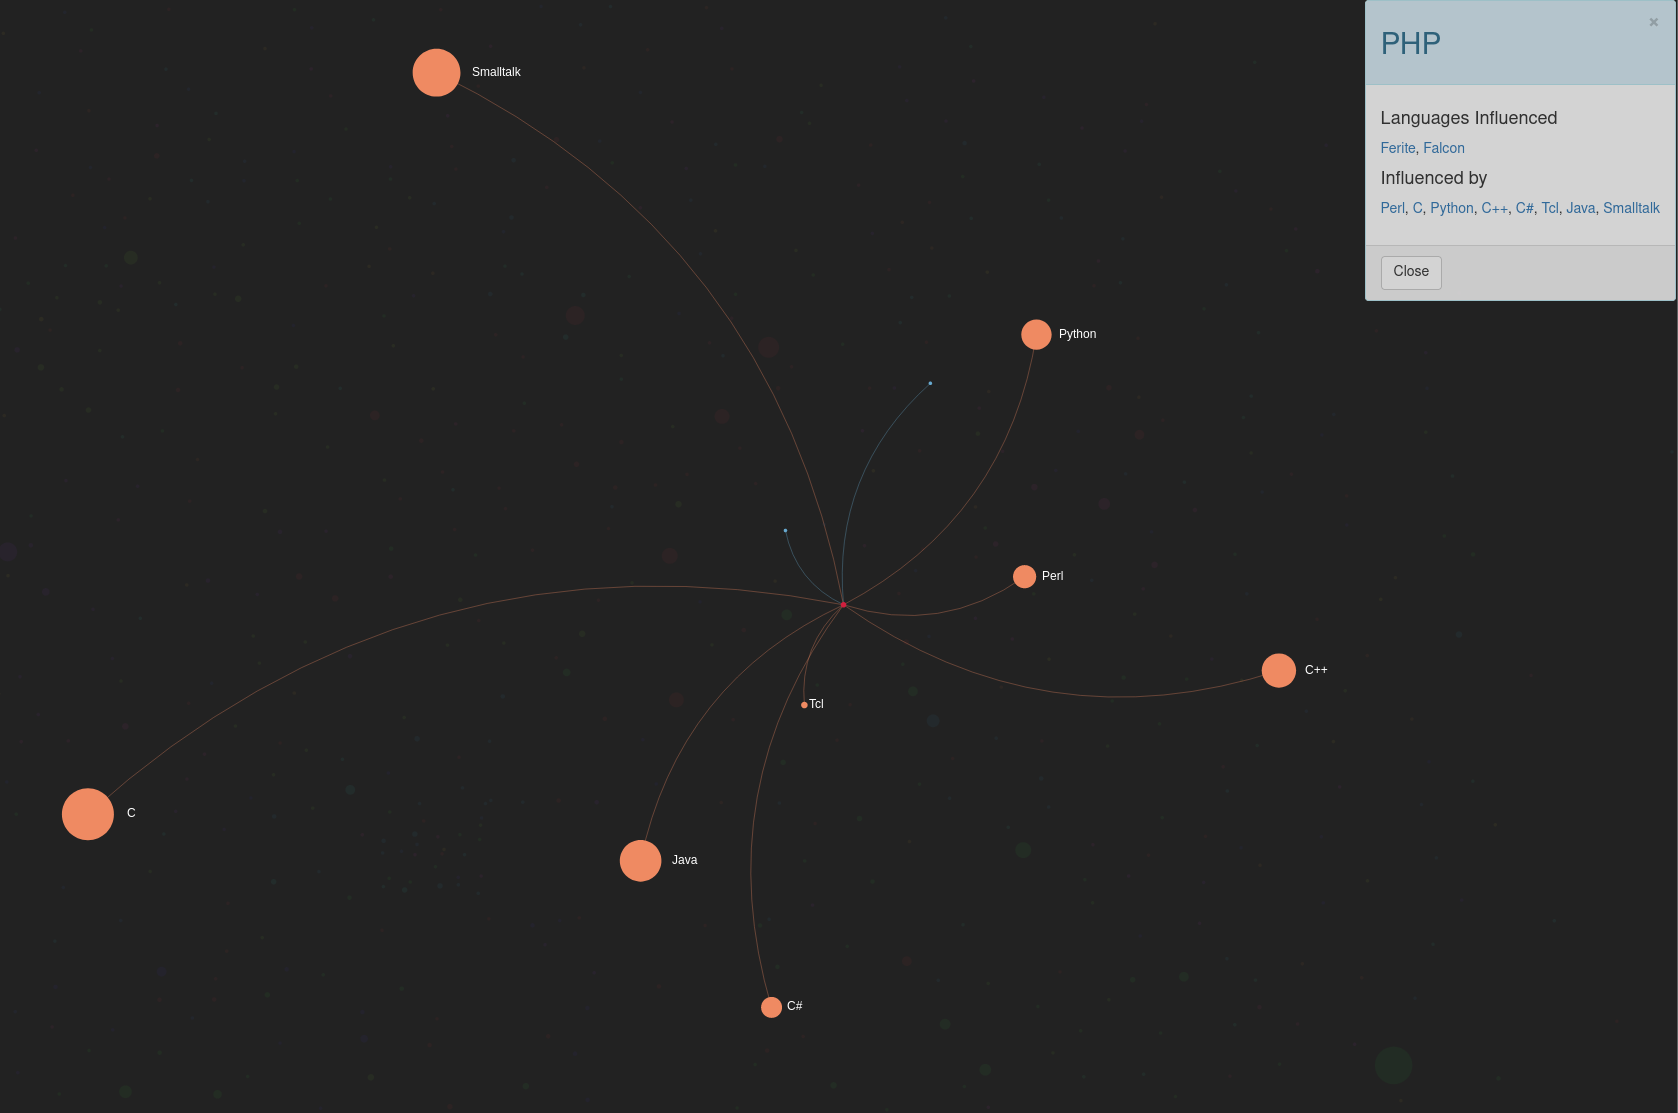
\includegraphics[width=\paperwidth, height=\paperheight]{src/session/history/resources/php.png}}

  \note[item]{
    This very brief history here shows which languages influenced PHP.
  }
  \note[item]{
    PHP has also influenced 2 languages...

  }
\end{frame}

% \begin{frame}{My cool three points}
%     \begin{itemize}
%       \item<1-|alert@1> Point 1
%       \item<3-|alert@3> Point 2
%       \item<5-|alert@5> Point 3
%     \end{itemize}
% \end{frame}
